\documentclass{beamer}

\usepackage{mjclectureslides}

\definecolor{Dblue}{rgb}{.255,.41,.884}

\title[Sets and Functions]
{Introduction to Analysis: \\
Sets and Functions}
%\author[Prof. Michael Carlisle]{Prof. Michael Carlisle}
%\institute{Baruch College, CUNY}
%\date{Fall 2017}
\date{}

\begin{document}

\frame{\titlepage}


\frame{ \frametitle{Set / Element}

We start with the basic definitions of set notation, as first written down by Georg Cantor (1845-1918). 


\begin{figure}[!ht]
  \centering
    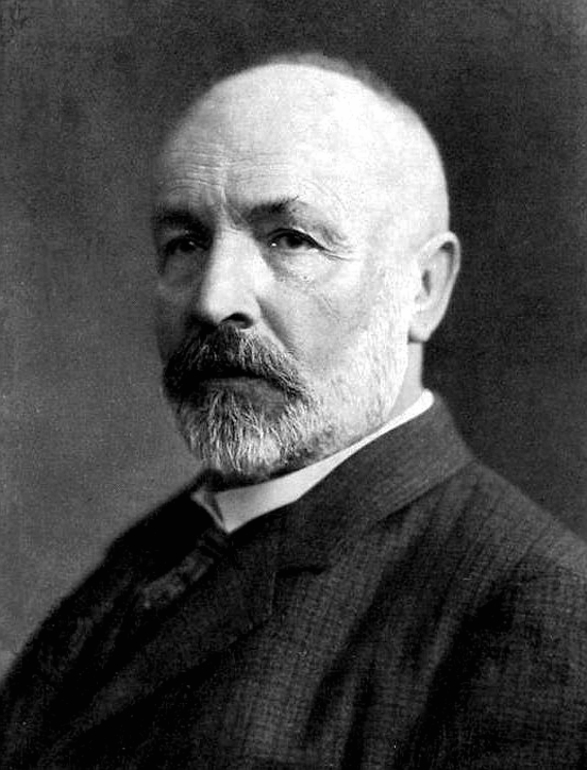
\includegraphics[width=2in]{georg-cantor.jpg}
\end{figure}


}


\frame{ \frametitle{Set / Element}


\vspace{5mm}

\begin{defn} A \textbf{set} is a collection of distinct objects, called the set's \textbf{elements}. 

\vspace{5mm}

The elements:
\begin{itemize}
\item do not necessarily have an inherent order or relationship to each other (although they usually will); 
\item duplicates are not allowed; 
\item they are merely \emph{different things in the same bag}. 
\end{itemize}
\end{defn}

}


\frame{ \frametitle{Set / Element Notation}

``The set $A$ contains three elements: 

\begin{center}
`cat', `tree', and the number 6.''
\end{center}

This is denoted 
\[ A = \{ \text{tree}, \text{cat}, 6 \} \]

\vspace{3mm}

with curly brackets indicating the set.

\vspace{5mm}

This is an \emph{explicit} definition of a particular set. It has 3 elements.

\vspace{5mm}

``6 is an element of $A$'' is denoted $6 \in A$.\\

\vspace{5mm}

``'dog' is not an element of $A$'' is denoted dog $\not \in A$. 

}



\frame{ \frametitle{Set / Element Notation}

``The set $B$ consists of the even numbers \emph{strictly} between 0 and 25'' 
(i.e. \emph{exclusive}) is an \emph{implicit} definition of the set denoted 

\vspace{3mm}

\[ B = \{ 2, 4, 6, ..., 22, 24\}. \]

\vspace{5mm}

The \emph{ellipsis} ``...'' means: 

\begin{center}
``we agree on, and you understand, the pattern given by context''.
\end{center}

}


\frame{ \frametitle{Set / Element Notation: ``Set Builder'' Notation}

Another way to write

\vspace{3mm}

\[ B = \{ 2, 4, 6, ..., 22, 24\} \]

\vspace{3mm}

is 

\vspace{3mm}

\[ B = \{ x \in \mathbb{Z} \, | \, 0 < x < 25, \, x \text{ even}\}, \]

\vspace{3mm}

where the vertical bar $|$ means ``such that''. 

\vspace{3mm}

(Sometimes a colon : is used instead of the bar $|$.)

}



\frame{ \frametitle{Popular Number Sets}

\[ \mathbb{N} = \{ 1, 2, 3, ... \} \]
 is the set of \textbf{natural} 
or \textbf{counting numbers} (sometimes with 0). 

\vspace{5mm}

\[ \mathbb{Z} = \{ ..., -3, -2, -1, 0, 1, 2, 3, ... \} \] 
is the set of \textbf{integers} (for the German word Zahlen (``numbers'')). 

\vspace{5mm}

\[ \mathbb{Q} = \left\{ \frac{m}{n} \, \bigg| \, m, n \in \mathbb{Z}, \, n \neq 0 \right\} \] 
is the \textbf{rational numbers} (fractions, ratios; Q for ``quotient''). 

}


\frame{ \frametitle{Real Number Sets}

$\mathbb{R}$ is the set of \textbf{real numbers}, containing all rational and irrational numbers. This is the set of numbers along the continuous number line, containing all infinite-length decimal expansions. 

\vspace{4mm}

\begin{figure}[!ht]
  \centering
    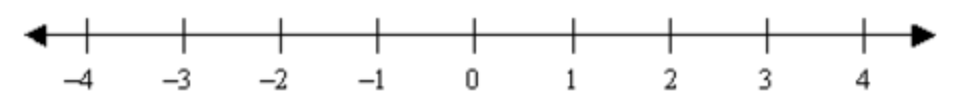
\includegraphics[width=4in]{numberline.png}
\end{figure}

\vspace{4mm}

Our focus in this course is sets, sequences, and functions on $\R$. 

}



\frame{ \frametitle{Intervals of Real Numbers}

\begin{figure}[!ht]
  \centering
    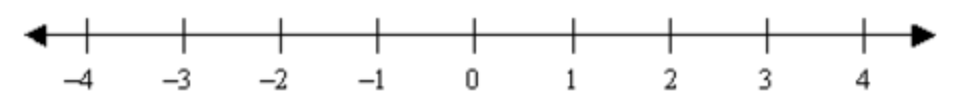
\includegraphics[width=4in]{numberline.png}
\end{figure}

\vspace{4mm}


An \textbf{open interval} of real numbers is denoted 
\[ (a, b) = \{ x \in \mathbb{R} : a < x < b \}. \]
(In some texts, notably French, open interval notation is $]a,b[$.)

\bigskip

A \textbf{closed interval} of real numbers is denoted 
\[ [a, b] = \{ x \in \mathbb{R} : a \leq x \leq b \}. \]

}


\frame{ \frametitle{Cardinality}

The \textbf{cardinality} of a set is the number of (distinct) elements of the set. 
The cardinality of the set $A$ is denoted $|A|$ or $\#A$. 

\vspace{5mm}

\textbf{Finite} sets have an obvious cardinality: count the elements. 

\vspace{5mm}

Examples: $|\{ 4, 6, 2, 9 \}| = 4$, $|\{ 7, 8, ..., 100 \}| = 94$. 

\vspace{5mm}


\textbf{Infinite} sets are more complicated to deal with. 

}



\frame{ \frametitle{Empty Set}

The \textbf{empty set} is the set with no elements (think: an empty bag). 

\vspace{5mm}

It is denoted 

\[ \emptyset \] 

and defined with curly brackets by 

\[ \emptyset = \{\}. \]

The cardinality of the empty set is 

\[ |\emptyset| = 0. \]

}


\frame{ \frametitle{Venn diagrams}

A \textbf{Venn diagram} (named after John Venn (1834-1923)) is a simple graphic displaying the overlap of different sets.

\vspace{5mm}

We use Venn diagrams to help understand problems in counting, probability, logic, and other fields. 

\vspace{5mm}

We'll sketch some diagrams for two sets $A$ and $B$, sharing the same universal set $U$ (the box surrounding them).

}


\frame{ \frametitle{Union}


Some basic operations we can use on sets are: 

\vspace{5mm}

The \textbf{union} of the sets $A$ and $B$ is the set of all elements of $A$ and $B$ combined. It is denoted $A \cup B$, and defined by 

\[ A \cup B = \{ x : \, x \in A \text{ or } x \in B \text{ (or both)}\}. \]

\begin{figure}[!ht]
  \centering
    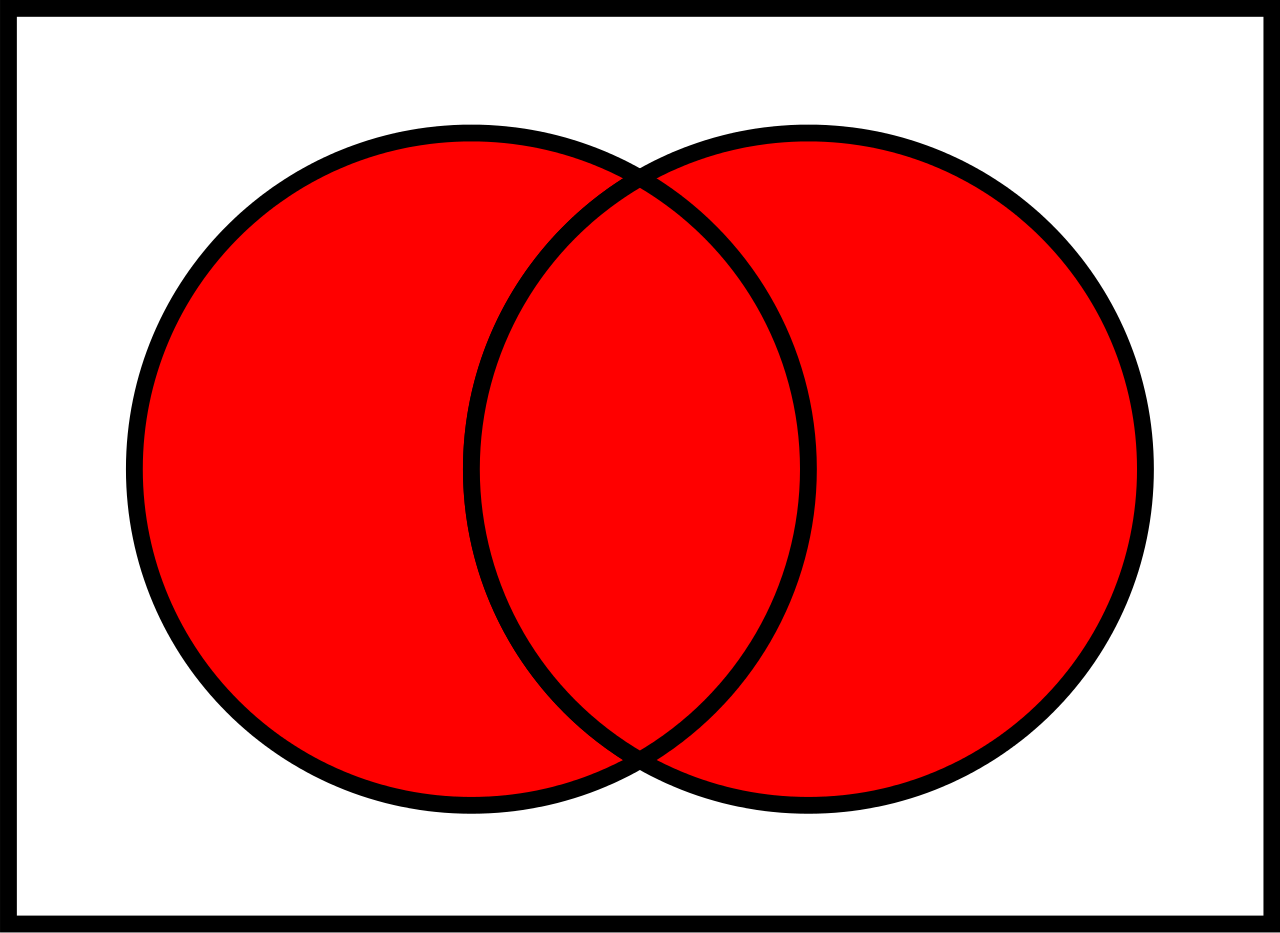
\includegraphics[width=2in]{union.png}
\end{figure}


}


\frame{ \frametitle{Intersection}

The \textbf{intersection} of the sets $A$ and $B$ is the shared elements of $A$ and $B$. It is denoted $A \cap B$ or $AB$, and defined by 

\[ A \cap B = \{ x : \, x \in A \text{ and } x \in B \}. \]

\begin{figure}[!ht]
  \centering
    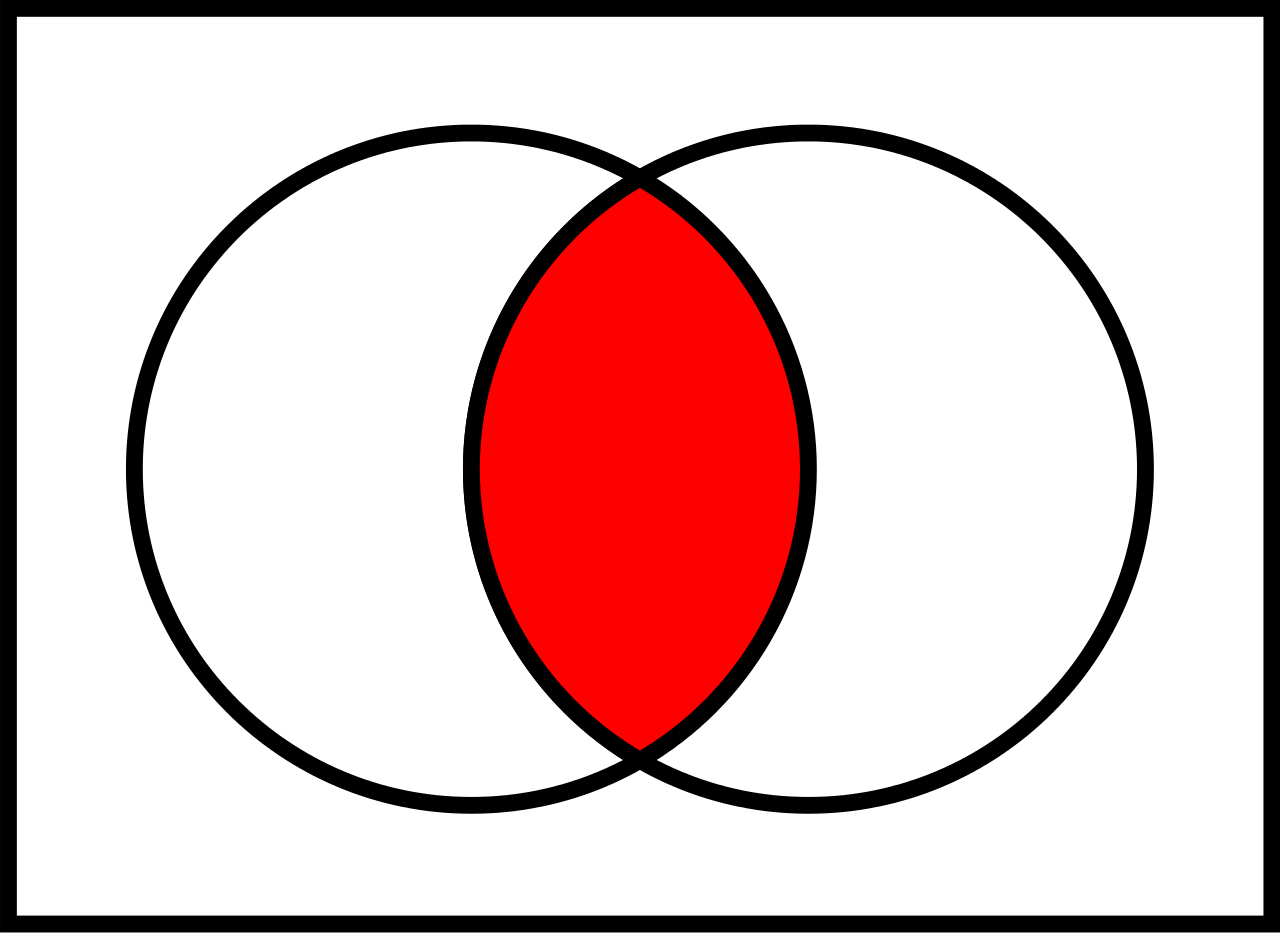
\includegraphics[width=2in]{intersection.png}
\end{figure}

If $A$ and $B$ have no common elements, we say $A$ and $B$ are \textbf{disjoint} sets and denote this fact by  $A \cap B = \emptyset$.

}



\frame{ \frametitle{Set Difference}

The \textbf{set difference} $B \setminus A$ (sometimes denoted $B - A$) is the elements of $B$ with the shared elements of $A$ removed. It is denoted 
\[ B \setminus A = \{ x : \, x \in B \text{ and } x \not \in A \}. \]

\begin{figure}[!ht]
  \centering
    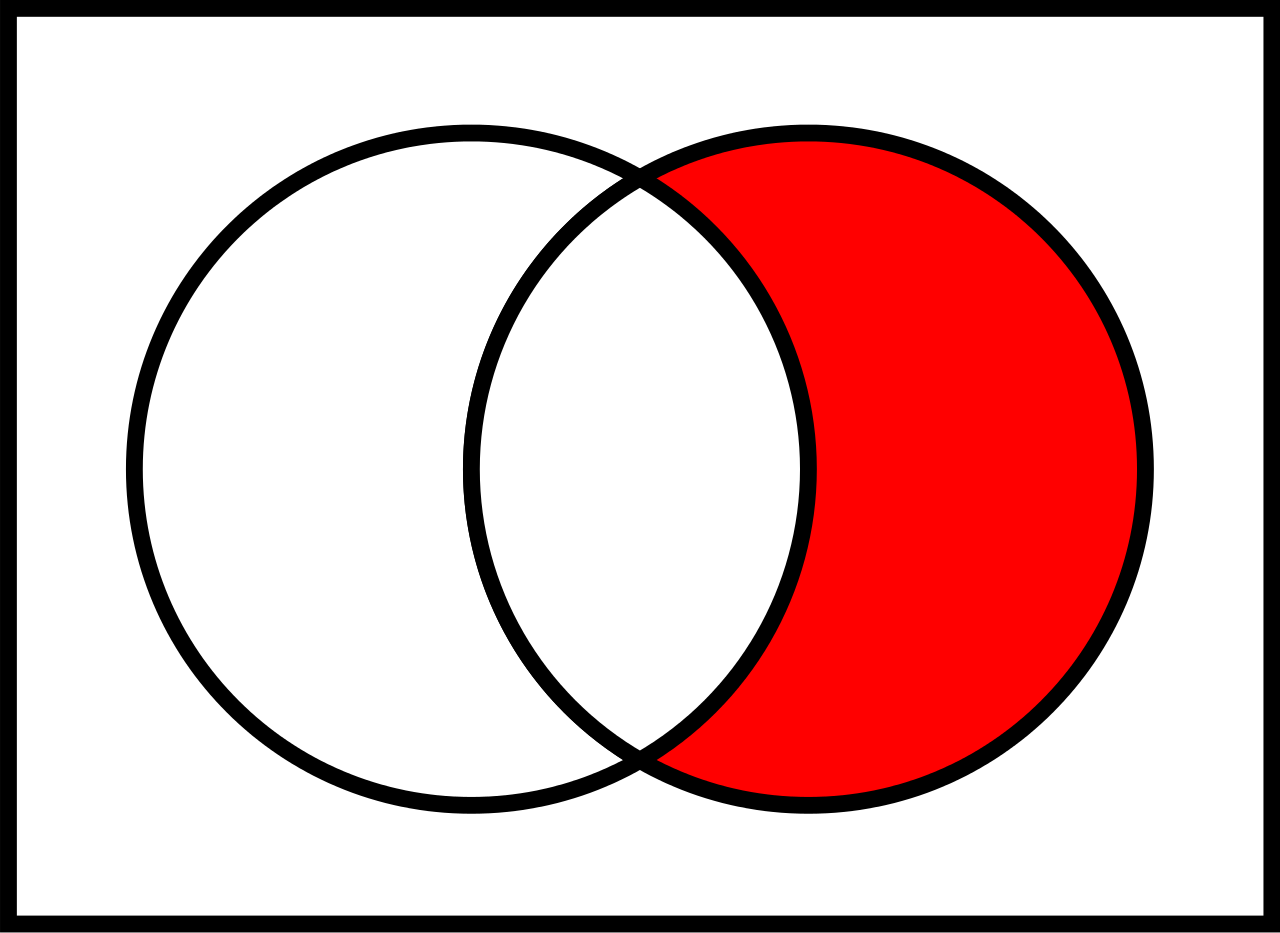
\includegraphics[width=2in]{BminusA.png}
\end{figure}

}


\frame{ \frametitle{Set Difference}

\[ A = \{ 1, 2, 5, 6, 7\}, \,\,\, B = \{ 2, 5, 8, 9, 13\} \]

\[ \implies A \setminus B = \{ 1, 6, 7\} \text{ but } B \setminus A = \{8, 9, 13\}. \]

\begin{figure}[!ht]
  \centering
    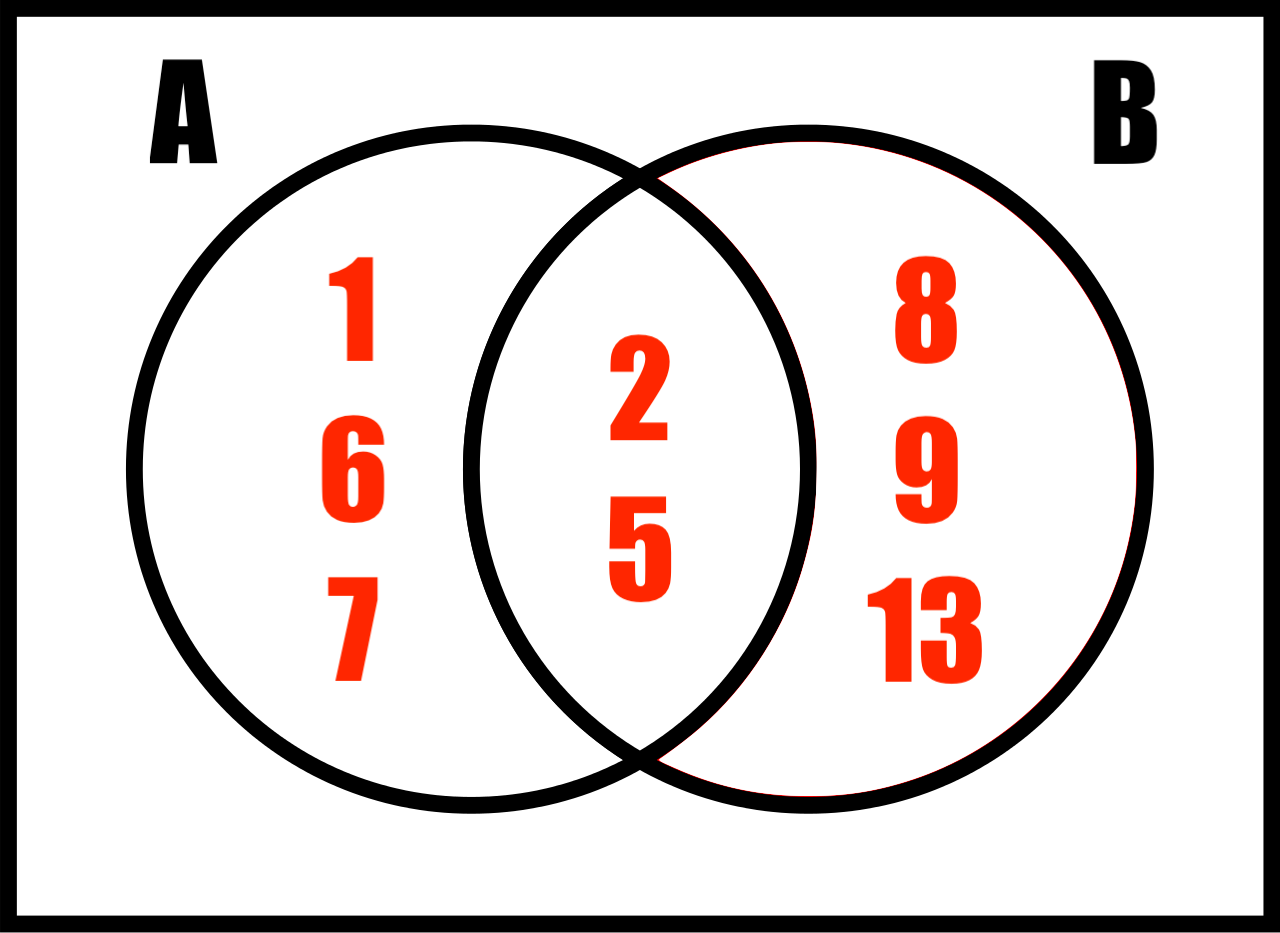
\includegraphics[width=2in]{BminusAexample.png}
\end{figure}

\begin{center}
Thus, $A \setminus B \neq B \setminus A$ (an important general result). 
\end{center}

}


\frame{ \frametitle{Subset}

The set $A$ is called a \textbf{subset} of $B$, denoted $A \subseteq B$, if all of $A$'s elements are in $B$. 
\[ A \subseteq B \iff (x \in A \implies x \in B). \]
\begin{figure}[!ht]
  \centering
    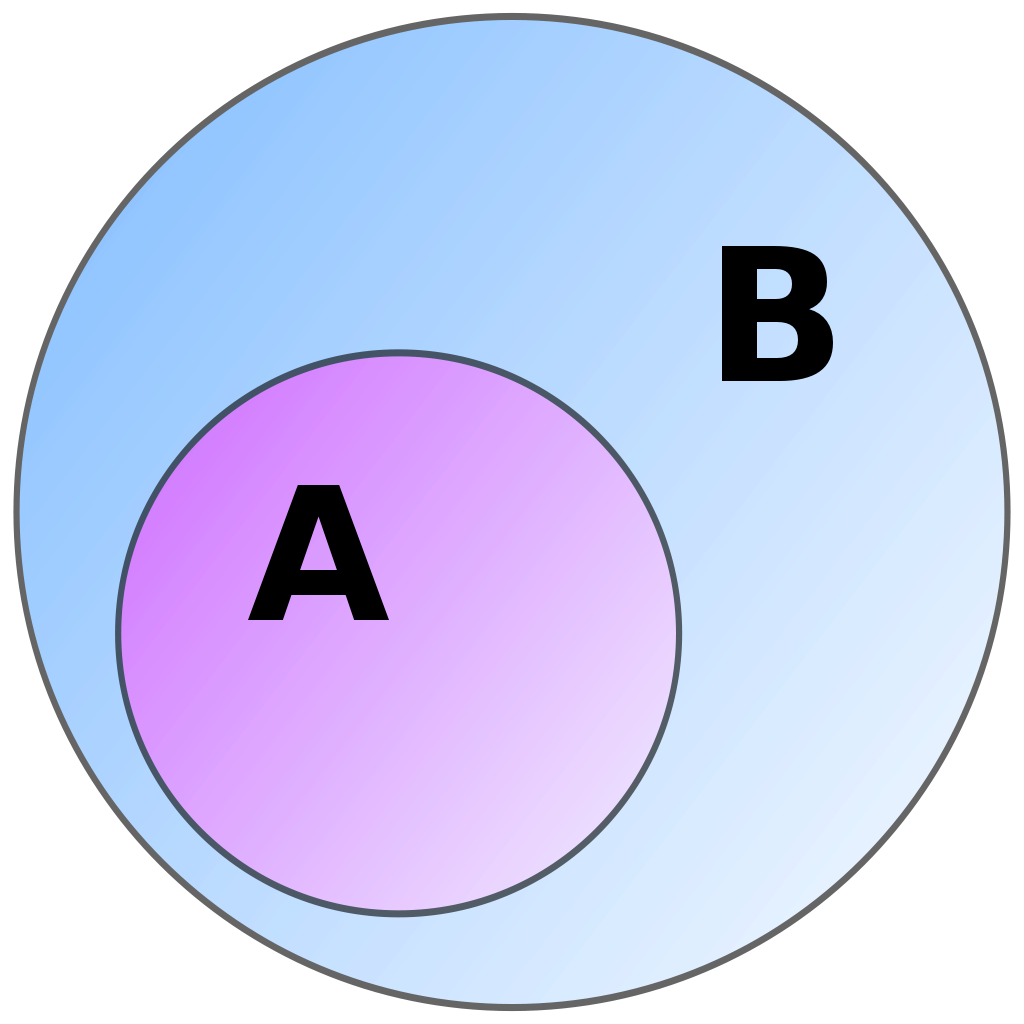
\includegraphics[width=2in]{AsubsetB.png}
\end{figure}

Two sets $A$ and $B$ are \textbf{equal} (written $A = B$) if $A \subseteq B$ and $B \subseteq A$.

}


\frame{ \frametitle{Universal Set, Complement}

In certain collections of problems, we may define a \textbf{universal set} as a common ``top-level set'' under which all the sets described in the problem are subsets of. 

\begin{figure}[!ht]
  \centering
    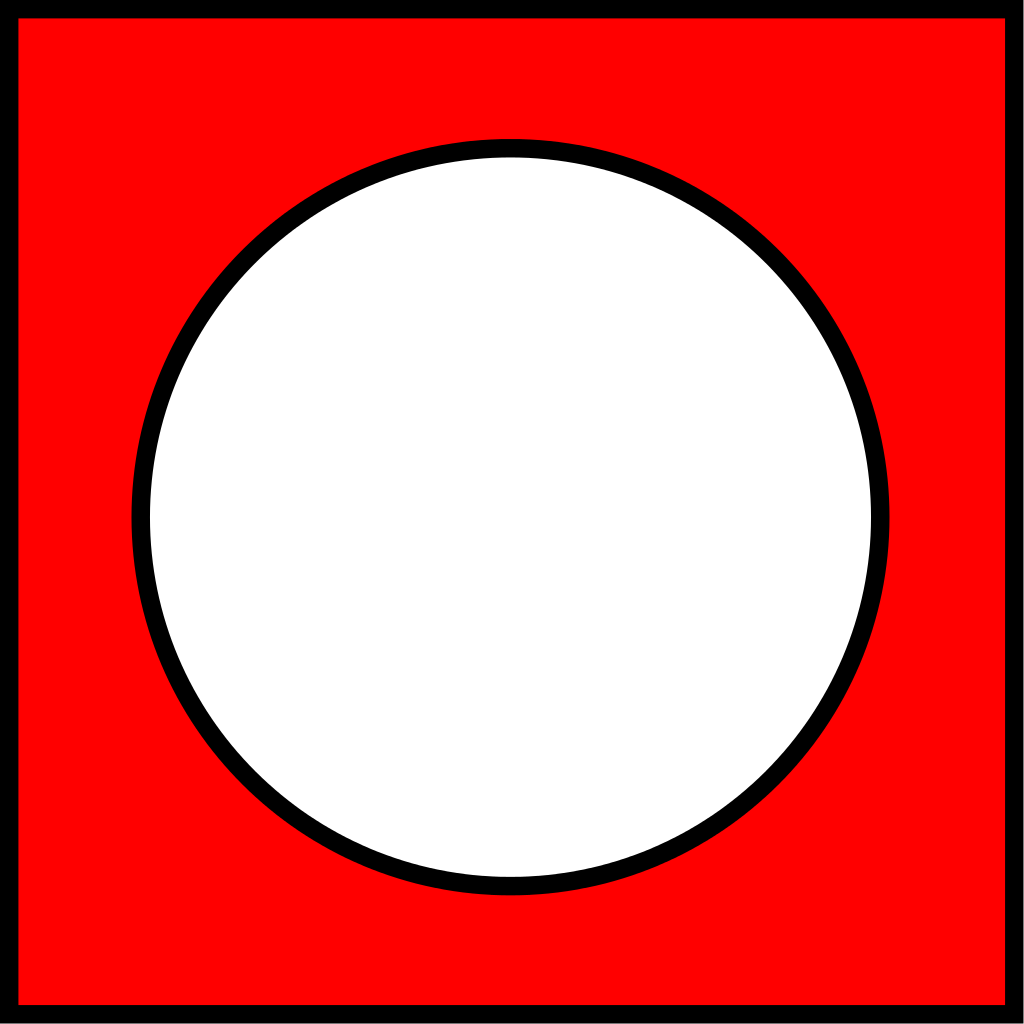
\includegraphics[width=2in]{Acomplement.png}
\end{figure}

}


\frame{ \frametitle{Universal Set, Complement}

The \textbf{complement} of a set $A$, relative to the universal set $U$, is denoted $A^C = U \setminus A$. (Some texts use $A'$ or $\overline{A}$.)

\begin{figure}[!ht]
  \centering
    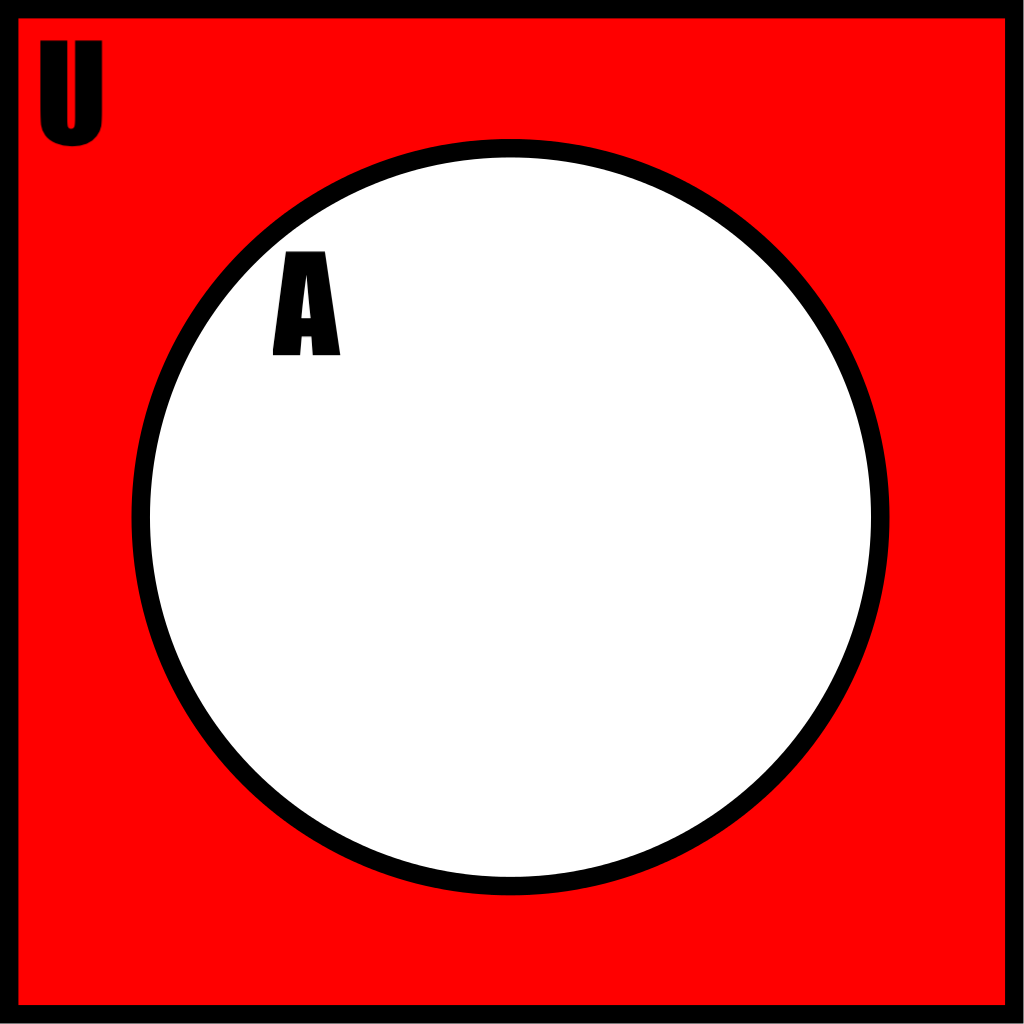
\includegraphics[width=2in]{Acomplement2.png}
\end{figure}

Using this, we can define the set difference as $A \setminus B = A \cap B^C$. 

}



\frame{ \frametitle{Example: intervals in $\R$}

Considering $\R = (-\infty, \infty)$ as the universal set\footnote{Note here that the ``infinity" symbol $\infty$ in this context means 
\begin{center}
``unbounded in this direction"
\end{center}
and is not itself representing a number.}, let 
\vspace{5mm}
\[ A = (1,\infty) = \{ x \in \R: x > 1\}. \]
\vspace{5mm}
Then 
\vspace{5mm}
\[ A^C = \R \setminus A = (-\infty, 1] = \{ x \in \R: x \leq 1\}. \]

}


\frame{ \frametitle{Unions, Intersections, Complements}

Union and intersection are \emph{commutative} operations: 

\vspace{5mm}

\[ A \cup B = B \cup A, \,\, A \cap B = B \cap A. \]

\vspace{5mm}

We've already seen that set difference is \emph{not} commutative: 

\vspace{5mm}

\[ A \setminus B \neq B \setminus A. \]

}


\frame{ \frametitle{Unions, Intersections, Complements}

Union and intersection are also \emph{associative}: 

\vspace{5mm}

\[ (A \cup B) \cup C = A \cup (B \cup C), \,\, (A \cap B) \cap C = A \cap (B \cap C). \]

\vspace{5mm}

Regardless of universal set, it should be clear that the complement of a complement is the original set: 

\vspace{5mm}

\[ (A^C)^C = A. \]

}


\frame{ \frametitle{Distributivity}

The \textbf{distributive property} describes how unions and intersections work together: 

\[ (A \cap B) \cup C = (A \cup C) \cap (B \cup C) \]

\[ (A \cup B) \cap C = (A \cap C) \cup (B \cap C) \]

}


\frame{ \frametitle{DeMorgan's Laws}

\textbf{DeMorgan's Laws} describe the complements of unions and intersections. Complementation flips a union or intersection: 

\[ (A \cap B)^C = A^C \cup B^C \]
\[ (A \cup B)^C = A^C \cap B^C \]

\vspace{3mm}

Note the similarity to DeMorgan's Laws in logic.

\vspace{5mm}

Visually, these rules make more obvious sense with Venn diagrams.

}



\frame{ \frametitle{Set (Cartesian) Product, Sequences}

The \textbf{Cartesian product} of two sets $A$ and $B$, denoted $A \times B$, is the set whose elements are \textbf{ordered pairs} $(a,b)$, where $a \in A$ and $b \in B$. (We will define $(a,b)$ set-theoretically later.)

\vspace{5mm}

Extending, the Cartesian product of $n$ sets $A_1, A_2, ..., A_n$, denoted $A_1 \times A_2 \times \cdots \times A_n$ or $\prod_{i=1}^n A_i$, is the set whose elements are \textbf{ordered $n$-tuples} $(a_1, a_2, ..., a_n)$, where $a_i \in A_i$ for $i=1,2,...,n$. 

\vspace{5mm}

If $A_1 = A_2 = \cdots = A_n = A$, we can write the product as $A^n$. 

\vspace{5mm}

Note that \emph{order matters} in a Cartesian product of sets: in general, 
\[ A \times B = B \times A \iff A = B. \]


}


\frame{ \frametitle{Power Set}

The \textbf{power set} of the set $A$, denoted $2^A$ or $\mathcal{P}(A)$, is the set of all subsets of $A$. (The notation will prove to be important.)

\vspace{5mm}

It is always true that $\emptyset, A \in 2^A$. 

\vspace{5mm}

\begin{ex}
$A = \{1, 4, 6\}$ has the power set 
\[ 2^A = \{ \emptyset, \{1\}, \{4\}, \{6\}, \{1,4\}, \{1,6\}, \{4,6\}, A\}. \]
\end{ex}

%\vspace{5mm}

The set $A$ has cardinality $|A| = 3$. 

\vspace{5mm}

The power set of $A$, $2^A$, has cardinality $|2^A| = 8$. 

}



\frame{ \frametitle{Example: Power Set}

For a finite set $A$ with cardinality $|A| = n$, what is $|2^A|$? 

\vspace{10mm}

In other words, how many possible subsets of $A$ are there?

}


\frame{ \frametitle{Example: Power Set}

For a subset $B \subseteq A$, consider the $n$ elements of $A$ in an order \\
(or, simply call them $1, 2, ..., n$). 

\vspace{10mm}

Build an ordered $n$-tuple of 1's and 0's via this ordering: 

\vspace{10mm}

For each element $x \in A$, place a 1 if $x \in B$, and 0 if $x \not \in B$. 

\vspace{10mm}

How many different ordered $n$-tuples of 1's and 0's are there? 

}


\frame{ \frametitle{Example: Power Set}


For example, let 
\[ B = \{ a, d \} \subseteq A = \{ a, b, c, d \}. \]

The $4$-tuple corresponding to $B$ is $(1,0,0,1)$. 

\vspace{10mm}

In general, 
\[ |\{0, 1\}^n| = |\{0,1\}|^n = 2^n. \]

\vspace{5mm}

The number of items in the power set $2^A$ is $|2^A| = 2^{|A|}$. 

}



\frame{ \frametitle{Some Proofs About Sets}

Two sets $A$ and $B$ are \emph{equal} (written $A=B$) if $A \subseteq B$ and $B \subseteq A$.

\vspace{5mm}

That is, 

\[ (x \in A \iff x \in B) \iff A = B. \]

\vspace{5mm}

Many proofs about sets are to show set equality. 

\vspace{5mm}

This means verifying the above iff statement.

}


\frame{ \frametitle{Some Proofs About Sets}

Much of modern mathematics is based in modern set theory.

\vspace{5mm}

To write a proof, you often need to deduce a set inclusion.

\vspace{5mm}

If $x$ is an element of the domain $D$ in question, $p(x)$ are the hypotheses, and $q(x)$ the conclusions, then you need to prove 

\[ x \in D \cap \{ y : \, p(y) \} \implies x \in D \cap \{ y : \, q(y) \}, \]

i.e.
\[ D \cap \{ y : \, p(y) \} \subseteq D \cap \{ y : \, q(y) \} \]
is the same statement as 
\[ \forall x \in D, \, p(x) \implies q(x). \]

}


\frame{ \frametitle{Proof of a Distributive Law of Sets}

\begin{prop} For sets $A$, $B$, $C$, 
\[ (A \cap B) \cup C = (A \cup C) \cap (B \cup C). \]
\end{prop}

\pf We need to prove 
\[ x \in(A \cap B) \cup C \iff x \in (A \cup C) \cap (B \cup C). \]

This is the conjunction of the two implications 
\[ x \in(A \cap B) \cup C \implies x \in (A \cup C) \cap (B \cup C) \]
and
\[ x \in(A \cap B) \cup C \Longleftarrow \, x \in (A \cup C) \cap (B \cup C). \]

}


\frame{ \frametitle{Proof of a Distributive Law of Sets}

Since the following argument goes both ways, we will write it with a chain of $\iff$s (to save space).

\vspace{5mm}

The argument shows the translation from set notation to logic and back in a cleverly-different form. 

\vspace{5mm}

Each step can be verified by checking the truth table for the pair of statements.
\begin{align*}
x \in(A \cap B) \cup C & \iff x \in A \cap B \text{ or } x \in C \\
 & \iff (x \in A \text{ and } x \in B) \text{ or } x \in C \\
 & \iff (x \in A \text{ or } x \in C) \text{ and } (x \in B \text{ or } x \in C) \\
 & \iff (x \in A \cup C) \text{ and } (x \in B \cup C) \\
 & \iff x \in (A \cup C) \cap (B \cup C). \,\,\, \blacksquare
\end{align*}

}



\frame{ \frametitle{Set (Cartesian) Product, Sequences}

The \textbf{Cartesian product} of two sets $A$ and $B$, denoted $A \times B$, \\
is the set whose elements are \textbf{ordered pairs}\footnote{This definition is by Kuratowski (1921).}
\[ (a,b) := \{ \{a\}, \{a, b\} \}, \] 
where $a \in A$ and $b \in B$.

\vspace{5mm}

\emph{Order matters} in a Cartesian product of sets: in general, 

\[ A \times B = B \times A \iff A = B. \]


}



\frame{ \frametitle{Binary Relations}

A \textbf{relation} $R$ (also known as a \textbf{correspondence} or \textbf{map}) \\from the set $A$ to the set $B$ is a subset of the product set $A \times B$. %, where elements are in the relation if they satisfy some property (which we also refer to by $R$). 

\vspace{5mm} 

The simplest notation for a binary relation is 
\[ R \subseteq  A \times B.\]

\vspace{5mm} 

Note that a relation has \textbf{ordering}: 

\begin{itemize}
\item $A$ is the first set in the Cartesian product \\(called the \textbf{domain} of $R$), and 
\item $B$ the second (called the \textbf{codomain} of $R$).
\end{itemize}

}



\frame{ \frametitle{Binary Relations: Notation}

An element being in a relation, $(a,b) \in R$, is often denoted by 

\[ aRb \text{ or } a \sim_R b. \] 

\vspace{5mm}

The notation 
\[ R: A \to B \]
is usually reserved for a special type of relation called a \emph{function}, that \emph{maps} ``from'' the set $A$ ``to'' the set $B$. In this case we will say that $a$ \textbf{maps to} $b$ under $R$ with the notation 
\[ a \mapsto b. \]

}



\frame{ \frametitle{Examples of Binary Relations}

Relations are the primary concept tying pieces of data together in \emph{relational databases}.

\vspace{3mm}

Here are some examples of relations: 

\vspace{3mm}

\begin{itemize}
%\item ``is an element of'': $\in$, from ``the set of all elements'' to ``the set of all sets'' (under ZFC, to avoid Russell's Paradox, etc.);
\item ``divides'': $| \subseteq \Z \times \Z$\\$(4,8) \in |$, i.e. $4 | 8$, $(6,3) \not \in |$, i.e. $6 \not | 3$;
\vspace{3mm}
\item ``$a$ teaches the course $b$, in Fall 2017, at Baruch College'': \\
from the set of all instructors to the set of all course offerings, containing
(``Michael Carlisle'', ``MTH 4010 CMWA'') \\
but not (``Michael Carlisle'', ``MTH 4000 JMWA'');
\vspace{3mm}
\item ``is greater than'': $> \, \subseteq \R \times \R$\\$(9.24,5) \in \, >$, i.e. $9.24 > 5$, but $(1,1.2) \not \in \, >$.
\end{itemize}

}



\frame{ \frametitle{Sets involved with a binary relation}

For a relation $R \subseteq A \times B$: 

\begin{itemize}
\item The \textbf{domain} is $A$. Not all elements of a domain of a relation need to map to elements in the codomain. 
\vspace{3mm}
\item The \textbf{codomain} is $B$. Not all elements of the codomain need to be mapped to by an element of the domain.
\vspace{3mm}
\item For any subset of the domain $C \subseteq A$, the \textbf{image} of $C$ under $R$ is the subset of $B$ defined by 
\[ R(C) = \{ b \in B: \, \exists a \in C, aRb \}. \]
\end{itemize}

}


\frame{ \frametitle{Sets involved with a binary relation}

For a relation $R \subseteq A \times B$: 

\begin{itemize}
\item The image of $A$ under $R$ is called the \textbf{range} of $R$: \\range($R$) = $R(A)$. 
\vspace{3mm}
\item For any subset of the range $D \subseteq B$, the \textbf{pre-image} (or \textbf{inverse image}) of $D$ under $R$ is the subset of $A$ defined by 
\[ R^{-1}(D) = \{ a \in A: \, \exists b \in D, aRb \} =  \{ a \in A: \, \exists b \in D, bR^{-1}a \}. \]
\end{itemize}

}



\frame{ \frametitle{Properties of Relations where domain = codomain}

Let $R \subseteq A \times A$. $R$ may have some of the following properties: 

\begin{itemize}
\item \textbf{reflexive}: $\forall x \in A$, $xRx$. \\
%(Every vertex in $G$ has a loop.)
\vspace{3mm}
\item \textbf{irreflexive}: $\forall x \in A$, $\lnot (xRx)$. \\
%(No vertex in $G$ has a loop.) \\
Note: $R$ cannot be both reflexive and irreflexive, \\
but $R$ could be neither. %(if some, but not all, $x$ have loops).
\vspace{3mm}
\item \textbf{symmetric}: $\forall x, y \in A$, $xRy$ $\implies$ $yRx$.\\
%(Every edge has a matching edge back.)
\vspace{3mm}
\item \textbf{antisymmetric}: $\forall x, y \in A$, $xRy$ and $yRx$ $\implies$ $x=y$.\\
%(The only matching edges are actually loops.)
\vspace{3mm}
\item \textbf{asymmetric}: $\forall x, y \in A$, $\lnot(xRy$ and $yRx)$.\\
%(No edges have matching edges back, and there are no loops.)
%\onslide<3->
\vspace{3mm}
\item \textbf{transitive}: $\forall x, y, z \in A$, $xRy$ and $yRz$ $\implies$ $xRz$.\\
%(Any path from one vertex to another is possible by one edge.)
\end{itemize}


}



\frame{ \frametitle{Equivalence Relations}

\begin{defn}
If a relation $R$ on one set $A$ is: 

\begin{itemize}
\item reflexive ($\forall x \in A$, $xRx$), 
\vspace{3mm}
\item symmetric ($xRy \implies yRx$), and 
\vspace{3mm}
\item transitive ($xRy, yRz \implies xRz$), 
\end{itemize}

then we call $R$ an \textbf{equivalence relation}. 

\vspace{5mm} 

The concept of ``equivalence relation'' generalizes the notion of ``equality'' to accept more concepts than ``is the same element''.
\end{defn}

}


\frame{ \frametitle{Equivalence Relations}

Some examples of equivalence relations: 

\begin{itemize}
\item usual equality $=$ \emph{on any set};
\vspace{3mm}
\item congruence \emph{modulo} $n$ on $\Z$; 
\vspace{3mm}
\item ``is in this classroom today'' \\
on the set of students in the school today.
\end{itemize}

}


\frame{ \frametitle{An Equivalence Relation Partitions a Set}

An equivalence relation $R \subseteq A \times A$ \emph{partitions} the set $A$ into \textbf{equivalence classes}, each of which has elements which are symmetric and transitive under $R$ (all are reflexive). 

\vspace{10mm}

The notation of an equivalence class is $[k]$ or $cl(k)$ for $k \in A$, representing \emph{all} elements of that class. 

}


\frame{ \frametitle{An Equivalence Relation Partitions a Set: Modulo}

\begin{ex}
Congruence modulo $n$ partitions $\Z$ into $n$ equivalence classes: 
\begin{align*}
[0] & = \{ ..., -2n, -n, 0, n, 2n, ... \} \\
& \\
[1] & = \{ ..., -2n+1, -n+1, 1, n+1, 2n+1, ... \} \\
 & ... \\
& \\
[n-1] & = \{ ..., -2n-1, -n-1, -1, n-1, 2n-1, ... \}.
\end{align*}
\end{ex}

%In the Markov process setting, an equivalence class is called a \textbf{communicating class} under ``can reach and be reached from''. 

}


\frame{ \frametitle{Real-Valued Functions of a Real Variable}

\begin{defn}
$f: D \to \R$ is a \textbf{real-valued function of a real variable} if 

\begin{itemize}
\item $f$ is a relation from $D$, its \textbf{domain} \\ (in this course, is a subset of $\R$ or $\R^n$), i.e. $dom(f) = D$, 
\vspace{3mm}
\item to $\R$, its \textbf{codomain}, i.e. $cod(f) = \R$, 
\vspace{3mm}
\item such that every point $x \in D$ has exactly one value $y \in \R$ \\such that $(x,y)$ is an element of $f$, \\i.e. $f$ is \textbf{well-defined} on its domain.
\end{itemize}
\end{defn}

}


\frame{ \frametitle{Real-Valued Functions of a Real Variable}

We use the \textbf{functional notation} to describe the values of $f$: 

\begin{itemize}
\item $x$ is typically used as the \textbf{independent variable}, or \textbf{argument}, from the domain, i.e. $x \in D$, and
\vspace{3mm}
\item $y = f(x)$ is the \textbf{dependent variable}, or \textbf{value} of $f$ at $x$.
\end{itemize}

\vspace{5mm}

The \textbf{image} of $f$ under the subset $C \subseteq D$ is the set of target outputs in the codomain $\R$ whose source inputs are in $C$: 
\[ f(C) =  \{ y \in \R \,\, | \,\, \exists x \in C, \,\, y = f(x) \}. \]
The \textbf{range} of $f$ is the image of the domain, $range(f) = f(D)$.


}


\frame{ \frametitle{Functions}

Certain types of functions bear their own names: 

\vspace{5mm}

\begin{itemize}
\item A \textbf{constant function} $f: A \to B$ maps every element $a \in A$ to the same element $b^* \in B$: $\forall a \in A$, $f(a) = b^*$.
\vspace{3mm}
\item An \textbf{identity function} $f: A \to A$ maps every element $a \in A$ to itself: $\forall a \in A$, $f(a) = a$. 
\end{itemize}

}


\frame{ \frametitle{Inverse Functions}

We use the notation $f^{-1}$ to refer to the inverse relation to the function $f:A \to B$. In general, $f^{-1}$ is not a function. 

\vspace{5mm}

If $f^{-1}$ is a function, then it is defined on $range(f) = f(A) \subseteq B$, \\we call it the \textbf{inverse function} of $f$, and the following hold.

\begin{itemize}
\item $f$ must be injective.
\vspace{3mm}
\item If $f(a) = b$, then $f^{-1}(b) = a$.
\vspace{3mm}
\item  $f(f^{-1}(b)) = b$ and $f^{-1}(f(a)) = a$ for every $a \in A$, $b \in f(A)$.
\end{itemize}

}


\frame{ \frametitle{Function Composition}

If $f: A \to B$ and $g:B \to C$ are functions, with $f(A) = g^{-1}(C)$, then define the \textbf{function composition} $g \circ f: A \to C$ by 

\[ (g \circ f)(a) = g(f(a)) = g(b) = c, \text{ if } f(a) = b \in B. \]

\vspace{5mm}

Note that $f \circ g \neq g \circ f$ unless $A = B = C$ and $f = g$. 

}


\frame{ \frametitle{Function Composition Properties}

\begin{itemize}
\item If $f$ and $g$ are injective, then so is $g \circ f$.
\vspace{3mm}
\item If $f$ and $g$ are surjective, then so is $g \circ f$.
\vspace{3mm}
\item Hence, if $f$ and $g$ are bijective, then so is $g \circ f$. 
\vspace{3mm}
\item If $f^{-1}$ is a function, then 
\[ f \circ f^{-1}: f(A) \to f(A) \] 
and 
\[ f^{-1} \circ f: A \to A \]
are identity maps.
\end{itemize}

}




\frame{ \frametitle{Cardinality}

The \textbf{cardinality} of a set is the number of (distinct) elements of the set. The cardinality of the set $A$ is denoted $|A|$. 

\vspace{5mm}

\textbf{Finite} sets have an obvious cardinality: count the number of elements. 

\vspace{5mm}

Examples: $|\{ 4, 6, 2, 9 \}| = 4$, $|\{ 7, 8, ..., 100 \}| = 94$. 

\vspace{5mm}

If two sets have the same cardinality, they are called \emph{equinumerous}. 

}


\frame{ \frametitle{Infinite Cardinality}

\textbf{Infinite} sets have more elements than any finite set. 

\vspace{5mm}

The first thing to know about infinite sets is: 

\begin{center}
\emph{There is an infinite hierarchy of sizes of infinity}.
\end{center}

}


\frame{ \frametitle{Infinite Cardinality: Countable, Uncountable}

The ``smallest'' level is called \textbf{countable} (the \emph{cardinal number} denoting this count is  $\aleph_0$); the next highest\footnote{if you believe a statement called the \emph{continuum hypothesis}} is 
\[ \aleph_1 = 2^{\aleph_0}, \]
and any $\aleph_k$ with $k \geq 1$ represent \textbf{uncountable} infinite cardinality.

\vspace{3mm}

We can prove: 
\[ |\mathbb{N}| = |\mathbb{Z}| = |\mathbb{Q}| = \aleph_0; \,\,\, |\mathbb{R}| = \aleph_1. \]

}


\frame{ \frametitle{What is cardinality?, set equivalence}

We want to generalize the concept of 

\begin{center}
``counting the elements of a set'' 
\end{center}
to more sets than just finite sets. 

\vspace{5mm}

The set $B$ has cardinality at least as large as another set $A$ if 
\[ \exists g: A \hookrightarrow B \] 
i.e. there exists a function $g$ that is 1-1 (called an \textbf{injection}\footnote{The notation $\hookrightarrow$ is sometimes used to denote that a function is 1-1.}).

\vspace{5mm}

We denote this fact by $|A| \leq |B|$. 

}


\frame{ \frametitle{What is cardinality?, set equivalence}

Likewise, $|A| \geq |B|$ if 
\[ \exists h: A \to B \] 
that is a \textbf{surjection} (onto). 

\vspace{5mm}

Two sets $A$ and $B$ are called \textbf{equivalent} (or \textbf{equinumerous}, or in \textbf{1-1 correspondence}), denoted in several ways: 
\[ A \sim B, \,\, A \approx B, \,\, |A| = |B|, \]
if $\exists$ a \textbf{bijection} (1-1, onto function) $f: A \to B$. 

}


\frame{ \frametitle{Power set}

Recall, the \textbf{power set} of a set $A$, denoted $\mc{P}(A)$ or $2^A$, is the set of all subsets of $A$: 
\[ 2^A = \{ E: \,\, E \subseteq A \}. \]
It should be clear that, since there is at least one more subset of $A$ than elements of $A$, that for finite sets $A$, $|2^A| > |A|$. In fact, 

\vspace{3mm}

\begin{thm}
$|2^A| > |A|$ for any set $A$. 
\end{thm}

\vspace{3mm}

We will prove this after we begin a discussion on infinite sets.

}



\frame{ \frametitle{Infinite sets}

A set whose cardinality is greater than $n$ for every $n \in \N$ is called an \textbf{infinite set}. 

\vspace{10mm}

The very obvious first example of this is $\N$ itself. 

}


\frame{ \frametitle{Infinite sets}

The cardinality of $\N$ is denoted $|\N| = \aleph_0$ (``aleph-null'', ``aleph-naught'', ``aleph-zero''), the \emph{first infinite cardinal}. 
 
\vspace{10mm}

Note that $\aleph_0$ is different from $\infty$ (``infinity''), the symbol representing unboundedness in a given direction. 

\vspace{10mm}

$\aleph_0$ refers to the infinite ``size'' of the set of natural numbers.  

\vspace{10mm}

A natural question is, what other sets are of size $\aleph_0$?

}



\frame{ \frametitle{Countable sets}

\begin{defn}
A set $S$ is called a \textbf{denumerable set}, or \textbf{countable set}\footnote{Sometimes finite sets are also called ``countable''; the term ``countably infinite'' is used to distinguish between the two types.}, or \textbf{denumerably (countably) infinite set}, if there is a 1-1 correspondence from $S$ to $\N$.
\end{defn}

\vspace{5mm}

All countably infinite sets are in the same equivalence class under the cardinality equivalence relation $\sim$ as $\N$. 

}


\frame{ \frametitle{Countable sets}

Two sets are equivalent if there exists a bijection between them. 

\vspace{5mm}

Thus, all countably infinite sets have bijections between all of them, just like, in the case of finite sets, all sets of size 5 have bijections between them all. 

\vspace{5mm}

The common concept is the \emph{list}. 

\vspace{5mm}

All sets of cardinality 5 have bijections with the set $\{1, 2, 3, 4, 5\}$, i.e. you can put the five elements on a numbered list. 

}



\frame{ \frametitle{Countable sets}

\begin{ex}
Let $A = \{1, 2, 3, 4, 5\}$, $B = \{a, b, c, d, e\}$, $C = \{3.4, \pi, 3e, \clubsuit, 0.4\}$. 
\end{ex}
Then $\exists f: A \to B$, $g: A \to C$ bijections, given by lists: 
\begin{enumerate}
\item $f(1) = a, g(1) = 3.4$
\item $f(2) = b, g(2) = 3e$
\item $f(3) = e, g(3) = 0.4$
\item $f(4) = d, g(4) = \pi$
\item $f(5) = c, g(5) = \clubsuit$
\end{enumerate}
is one possible pair of such bijections. \\
(How many bijections are there for each map?)

\vspace{3mm}

Infinite sets may be a bit less intuitive.

}



\frame{ \frametitle{Countable sets are, at first, unintuitive.}

A countable set's elements can be put on an infinitely-long list. 

\begin{prop}
$A = \{2, 3, 4, ...\} \sim \N$. 
\end{prop}

\vspace{5mm}

\pf $f: A \to \N$, defined by $f(n) = n-1$, is a bijection. \,\, $\blacksquare$

\vspace{5mm}

Thus, we cannot say that $A$ has ``one less element'' than $\N$; they have the \emph{same} cardinality $|A| = |\N| = \aleph_0$, both countably infinite.

}



\frame{ \frametitle{Countable sets are, at first, unintuitive. You get used to it.}

\begin{prop}
The positive evens $B = \{2, 4, 6, 8, ...\} \sim \N$. 
\end{prop}

\vspace{5mm}

\pf $f: B \to \N$, defined by $f(n) = n/2$, is a bijection. \,\, $\blacksquare$

\vspace{5mm}

Another: $g: \N \to B$, defined by $g(n) = 2n$, is a bijection.  \,\, $\blacksquare$

\vspace{5mm}

Thus, we cannot say that $B$ has ``half the elements'' of $\N$; they have the \emph{same} cardinality $|B| = |\N| = \aleph_0$, both countably infinite.

%\vspace{3mm} 

%\textbf{Arithmetic with infinite cardinals:}
%\[ k \in \N \implies \aleph_0 \cdot k = \aleph_0, \,\, \aleph_0 \div k = \aleph_0 \]

}



\frame{ \frametitle{Countable sets are, at first, unintuitive. You get used to it.}

\begin{prop}
$\Z$ is countable. 
\end{prop}

\vspace{5mm}

\pf $f: \N \cup \{0\} \to \Z$, defined by a ``hopping back and forth'' pattern: 

\[ f(n) = \left\{  \begin{array}{cl} \frac{n}{2} & n \text{ even} \\ -\frac{n+1}{2} & n \text{ odd} \end{array}\right. \]

\vspace{3mm}

is a bijection. Hence, $|\N \cup \{0\}| = |\Z|$. 

\vspace{3mm}

We can easily show that $|\N| = |\N \cup \{0\}|$ via the bijection $g: \N \to \N \cup \{0\}$ defined by $g(n) = n-1$. \,\, $\blacksquare$

}


\frame{ \frametitle{Countable sets are, at first, unintuitive. You get used to it.}

\begin{prop}
If $A_1$, $A_2$, ..., $A_n$ are countable sets, then their union $\bigcup_{i=1}^n A_i$ is also a countable set.
\end{prop}

\vspace{5mm} 

\pf Without loss of generality (Wlog), we assume all the elements of all $n$ sets are distinct. If not, discard duplicates.

\vspace{5mm}

Since each $A_i$ is countable, we can list the elements: 
\[ A_i = \{ a_{i1}, a_{i2}, a_{i3}, ... \}. \]
Therefore, we can merge all $n$ lists into one big list, showing that the union of the $n$ sets is also countable: 
\begin{align*}
\bigcup_{i=1}^n A_i = \{ & a_{11}, a_{21}, a_{31}, ...,  a_{n1}, a_{21}, a_{22}, a_{32}, ..., a_{n2}, 
  a_{31}, a_{32}, a_{33}, ... \}. \,\, \blacksquare
\end{align*}


}


\frame{ \frametitle{Countable sets are, at first, unintuitive. You get used to it.}

\begin{cor}
If $A \subseteq B \subseteq C$ and $|A| = |C|$, then $|A| = |B| = |C|$.
\end{cor}

\vspace{10mm}

\begin{prop}
The Cartesian product $\Z \times \Z$ is countable.
\end{prop}

\vspace{3mm}

\pf (sketch) There is a bijection $f: \N \to \Z \times \Z$ which can be visualized by drawing a spiral from the center of the coordinate plane outward, connecting all the points on the \emph{integer lattice}. \,\, $\blacksquare$

\vspace{5mm}

%\textbf{Arithmetic with infinite cardinals:}
%\[ |\Z \times \Z| = |\Z| \cdot |\Z| = \aleph_0 \cdot \aleph_0 = \aleph_0 = |\N| \]

}


\frame{ \frametitle{Countable sets are, at first, unintuitive. You get used to it.}

\begin{prop}
If $A$ and $B$ are countably infinite or finite, then the Cartesian product $A \times B$ is countable or finite. 
\end{prop}

\vspace{3mm}

\pf Obviously, if both $A$ and $B$ are finite, with $|A| = m$ and $|B| = n$, then $|A \times B| = mn$ is also finite.

\vspace{3mm}

If both $A$ and $B$ are countable, we can list their elements: 
\[ A = \{a_1, a_2, a_3, ... \}, \,\,\, B = \{b_1, b_2, b_3, ... \}. \]
We can list the elements of the Cartesian product ``diagonally'':
%, running through the sum of indices = 2, then the sum of indices = 3, and so on: 
\begin{align*} 
A \times B = \{ & (a_1, b_1), \\
 & (a_1, b_2), (a_2, b_1), \\
 & (a_1, b_3), (a_2, b_2), (a_3, b_1), ... \}. \blacksquare 
\end{align*}

}



\frame{ \frametitle{Countable sets are, at first, unintuitive. You get used to it.}

\begin{prop}
$\Q$ is countable.
\end{prop}

\vspace{3mm}

\pf (sketch) We can put $\Q$ in 1-1 correspondence with a subset $Q \subseteq \Z \times \Z$: 
\[ Q = \left\{(m, n): m, n \in \Z, \, \frac{m}{n} \in \Q \text{ and in lowest terms}\right\}. \]
Since $\Z \times \Z$ is countable by the previous theorem, and 
\[ \N \times \{1\} \subseteq Q \subseteq \Z \times \Z, \]
then, since $|\Q| = |Q|$, we have 
\[ \aleph_0 = |\N \times \{1\}| \leq |\Q| \leq |\Z \times \Z| = \aleph_0 \implies |\Q| = \aleph_0. \,\, \blacksquare \]

%First, we claim a bijection between $\Q = \{ \frac{m}{n}: \, m, n \in \Z, \, n \neq 0\}$ and the set $Q = \{(m, n): m, n \in \Z, \, \frac{m}{n} \in \Q \text{ and in lowest terms}\}$, giving us $|\Q| = |Q|$. Next, we show a bijection between $Q$ and $\Z \times \Z$ by using the spiral mentioned previously, skipping the points that are duplicated because an equivalent fraction has already been claimed (and $Q$ only contains the integer pairs representing lowest terms fractions). In this sense, since we ``skip some points'' of the integer lattice, $\N \times \{1\} \subseteq Q \subseteq \Z \times \Z$, and so by the above proposition, since $|\N| = |\N \times \{1\}| = |\Z \times \Z| = \aleph_0$, then $|Q| = |\Q| = \aleph_0$. \,\, $\blacksquare$

}


\frame{ \frametitle{Power set is strictly bigger (finite set)}

\begin{thm}
For a finite set $A$, $|A| < |2^A|$.
\end{thm}

\vspace{3mm}

\pf 
\[ |A| = n \in \N \implies 2^{|A|} = |2^A| = \sum_{j=0}^n {n \choose j} = 2^n > n = |A|. \,\, \blacksquare \]


}


\frame{ \frametitle{Power set is strictly bigger (any set)}

For infinite sets, however, we need a bit more work. 

\begin{thm}
$|A| < |2^A|$ for any set $A$. 
\end{thm}

\vspace{5mm}

\pf There is an injection 
\[ g: A \hookrightarrow 2^A \] 
defined by selecting singleton sets:  
\[ a \mapsto g(a) = \{a\}. \]
Therefore, $|A| \leq |2^A|$. 

}


\frame{ \frametitle{Power set is strictly bigger}

We need to show that \emph{no} bijection exists between $A$ and $2^A$; hence, 
\[ |A| \neq |2^A|. \]

\vspace{10mm}

We prove by contradiction. Assume $f: A \to 2^A$ is a bijection. 

\vspace{5mm}

We will show that no such $f$ can exist.

}


\frame{ \frametitle{Power set is strictly bigger}

If such an $f$ exists, then, for each $a \in A$, 

\vspace{5mm}

\begin{itemize}
\item either $a \in f(a)$ (which happens with $f(a) = A$),
\vspace{5mm}
\item or $a \not \in f(a)$ (which happens with $f(a) = \emptyset$),
\end{itemize}

\vspace{5mm}

but not both.

}


\frame{ \frametitle{Power set is strictly bigger}

Let 
\[ B = \{ b \in A: \, b \not \in f(b) \}. \] 

\vspace{3mm}

Then $B \subseteq A$ (and so $B \in 2^A$), since $B$ is well-defined if $f$ exists.

\vspace{5mm}

Since $B \in 2^A$, $\exists c \in A$ such that $B = f(c)$ since $f$ is a bijection. 

\vspace{5mm}

Is $c \in B$? By definition, if $c \in B$, then $c \not \in f(c) = B$. 

\vspace{3mm}

If $c \not \in f(c) = B$, then $c \in B$. This is a contradiction. $\contra$

\vspace{10mm}

Hence, there is no bijection between $A$ and $2^A$, and $|A| \neq |2^A|$. \,\, $\blacksquare$

}


\frame{ \frametitle{Cantor diagonalization argument}

The next proof is known as \textbf{Cantor's diagonalization argument}\footnote{Cantor published this argument in 1891. Bertrand Russell modified Cantor's diagonalization argument ten years later to show a weakness in Cantor's ``naive'' set theory, creating what is known as the ``barber paradox''.}, named after the use of the \emph{diagonal} 
\[ \{(c, f(c)):  c \in A \}. \]

An immediate consequence of this theorem is that there exists a hierarchy of ``sizes of infinity'': since $|A| < |2^A|$ for any set $A$, then $|\N| < |2^{\N}|$, and since $2^{\N}$ is itself a set, we have 
\[ |\N| < |2^{\N}| < |2^{2^{\N}}| < \cdots .\]

}



\frame{ \frametitle{$|\R| =$ ?}

What is the cardinality of the real numbers $\R$? 

\vspace{5mm}

Certainly, $|\R| \geq \aleph_0$, since $\Z \subseteq \R$. 

\vspace{5mm}

We can find the cardinality of $\R$ by finding a bijection between $\R$ and another set. 

\vspace{5mm}

That set is $2^{\N}$. 

}



\frame{ \frametitle{Uncountable sets}

We will define $\aleph_1 = |\R|$. We know $\aleph_0 \leq \aleph_1$.

\vspace{3mm}

How big is $\aleph_1$ relative to $\aleph_0$? 

\[ \aleph_0 = \aleph_1? \,\,\,\,\, \aleph_0 < \aleph_1? \]

\vspace{3mm}

If it turns out that $\aleph_0 < \aleph_1$, are there any cardinals between them?

\vspace{5mm}

We call sets of cardinality $\aleph_1$ or greater \textbf{uncountable sets}. 

\vspace{3mm}

Why we use that term will be explored shortly.

%\vspace{3mm}

%\textbf{Arithmetic with infinite cardinals:}
%\[ \aleph_0 < \aleph_1 \]
%\[ j, k \leq \aleph_0 \implies \,\, k\aleph_1 + j\aleph_0 = \aleph_1 \]


}



\frame{ \frametitle{Uncountable sets are weirder.}

We call a set $A$ 

\begin{itemize}
\item \textbf{finite} if we can list its elements on a finite-length list, \\
i.e. $\exists$ a bijection between $A$ and $\{1, 2, ..., n-1, n\}$. 

\vspace{3mm}

In this case, $|A| = n$. 

\vspace{5mm}

\item \textbf{countable} if we can list its elements on an infinite-length list, \\
i.e. $\exists$ a bijection between $A$ and $\N$.

\vspace{3mm}

In this case, $|A| = \aleph_0$. 

\vspace{5mm}

\item \textbf{uncountable} if no bijection exists between $A$ and any subset of $\N$. 

\vspace{3mm}

In this case, $|A| > \aleph_0$. 
\end{itemize}

}


\frame{ \frametitle{$|\R| > |\N|$ and all open intervals are the same cardinality}

\begin{thm}
$\R$ is uncountable, and any open interval $(a,b)$ has the same cardinality as $\R$: $|(a,b)| = |\R|$ for any $a, b \in \R$, $a < b$. 
\end{thm}

\vspace{5mm}

\pf There are many ways to write down this argument: \\
I will choose one that is visually easy to understand. 

\vspace{5mm}

First, we will start by showing that any open interval has the same cardinality as the open unit interval $(0,1)$. 

}


\frame{ \frametitle{$|\R| > |\N|$ and all open intervals are the same cardinality}

For $a, b \in \R$, $a < b$, the function $g: (a,b) \to (0,1)$ defined by 

\[ g(x) = \frac{x-a}{b-a} \] 

is a bijection (a line segment). Thus, $|(0,1)| = |(a,b)|$.

\vspace{5mm}

The function $h: (0,1) \to \R$ defined by 

\[ h(x) = \tan\left( \frac{(2x-1)\pi}{2} \right) \] 

is also a bijection, so $|(0,1)| = |\R|$. 

}


\frame{ \frametitle{Cantor's diagonalization argument: $|\R| > |\N|$}

Now, we will show that the open unit interval $(0,1)$ is uncountable. 

\vspace{5mm}

For a contradiction, assume $b: \N \to (0,1)$ is a bijection. 

\vspace{5mm}

Then $(0,1)$ is countable, so there is a list of the elements of $(0,1)$, which can be written as infinite-length decimal expansions: 
\begin{align*}
b(1) & = 0.a_{11} a_{12} a_{13} a_{14} a_{15} ... \\
b(2) & = 0.a_{21} a_{22} a_{23} a_{24} a_{25} ... \\
b(3) & = 0.a_{31} a_{32} a_{33} a_{34} a_{35} ... \\
b(4) & = 0.a_{41} a_{42} a_{43} a_{44} a_{45} ... \\
b(5) & = 0.a_{51} a_{52} a_{53} a_{54} a_{55} ... \\
...
\end{align*}
where the $a_{ij} \in \{ 0, 1, 2, ..., 8, 9 \}$. 
%(Note that we could use any other number base here, and the argument would be the same.)

}



\frame{ \frametitle{Cantor's diagonalization argument: $|\R| > |\N|$}

From this list, select the \emph{diagonal} digits and construct the number 

\[ a = 0.b_1 b_2 b_3 b_4 b_5 ... \]

where $b_j = (a_{jj} + 1)\mod 10$ for $j=1,2,3,4,...$. 
\begin{align*}
b(1) & = 0.\color{red}{a_{11}} \color{black}{a}_{12} a_{13} a_{14} a_{15} ... \\
b(2) & = 0.a_{21} \color{red}{a_{22}} \color{black}{a}_{23} a_{24} a_{25} ... \\
b(3) & = 0.a_{31} a_{32} \color{red}{a_{33}} \color{black}{a}_{34} a_{35} ... \\
b(4) & = 0.a_{41} a_{42} a_{43} \color{red}{a_{44}} \color{black}{a}_{45} ... \\
b(5) & = 0.a_{51} a_{52} a_{53} a_{54} \color{red}{a_{55}} \color{black}{...}  \\
...
\end{align*}
$a \neq b(j)$ for any $j$, i.e. $a$ is not on the list, since $a$ differs from $b(j)$ on digit $j$ of its expansion. Hence, $b$ is not a bijection. $\contra$ Therefore, $|\R| = |(0,1)| > |\N|$.  
\,\, $\blacksquare$
}


\frame{ \frametitle{A quick list of diagonal contradiction arguments}

In fact, we know 
\begin{thm}
$\aleph_1 = |\R| = |2^{\N}| = 2^{|\N|} = 2^{\aleph_0}$. 
\end{thm}
but will not prove this here.

}


\frame{ \frametitle{A quick list of diagonal contradiction arguments}

Here is a short list of important diagonal contradiction arguments: 

\vspace{5mm}

\begin{itemize}
\item Cantor (1891): $|\R| > |\N|$
\item Russell (1901): Russell's Paradox
\item G\"odel (1931): Incompleteness Theorems
\item Turing (1936): Entscheidungsproblem (Halting Problem)
\item Tarski (1936): Undefinability Theorem
\end{itemize}

\vspace{5mm}

The use of a diagonal-style contradiction proof is rooted in \emph{self-reference} in the key object constructed to make the contradiction. 

}


\end{document}
